\documentclass{article}
\usepackage[utf8]{inputenc}
\usepackage{amsmath}
\usepackage{mathrsfs}
\usepackage{amssymb}
\usepackage{amsfonts}
\usepackage{tikz}
\usepackage[margin=1in,headheight=13.6pt]{geometry}
\usepackage{amsthm}
\theoremstyle{definition}
\newtheorem{definition}{Definition}[section]
\theoremstyle{thrm}
\newtheorem{thrm}{Theorem}[section]
\theoremstyle{lma}
\newtheorem{lma}{Lemma}[section]
\theoremstyle{ppst}
\newtheorem{ppst}{Proposition}[section]
\theoremstyle{crlr}
\newtheorem{crlr}{Corollary}[section]
\usepackage{graphicx}
\renewcommand{\baselinestretch}{1.5}
\newenvironment{rcases}
  {\left.\begin{aligned}}
  {\end{aligned}\right\rbrace}
\usepackage{color}  
\usepackage{hyperref}
\hypersetup{
    colorlinks=true
    linktoc=all
    linkcolor=blue
}
\usepackage{fancyheadings}
\pagestyle{fancyplain}
\fancypagestyle{plain}{
\renewcommand{\headrulewidth}{0.4pt}
}
\lhead{\fancyplain{Haoyue(Heather) Tan}{Haoyue(Heather) Tan}}
\rhead{\fancyplain{STA347 lecture Notes}{STA347 Lecture Notes}}
\title{STA347 Probability - Lecture notes}
\author{Heather Tan}
\date{Sep - Dec 2019}
\begin{document}

\maketitle	
\tableofcontents
\pagebreak

\section{List of Common Sets}
\begin{itemize}
	\item Natural Number: $\mathbb{N} = \{1,2,\cdots\}$
	\item Whole: $\mathbb{W} = \{\mathbb{N}\} \cup \{0\}$
	\item Integers: $\mathbb{Z} = \{0, \pm1, \pm2,\cdots\}$
	\item Rationals: $\mathbb{Q} = \{\frac{n}{m}  | n \in \mathbb{Z}, m \in \mathbb{N}\}$
	\item Reals: $\mathbb{R} = \{x = \lim_{n\to\infty} r_n | r_n \in \mathbb{Q}, n \in \mathbb{N}\}$
	\item Complex: $\mathbb{C} = \{z = x+iy|x,y\in \mathbb{R}\}$
\end{itemize}
\section{Sequence of Event $A_n$}
\subsection{sigma-additivity}
\begin{definition}
	P is said to be $\sigma-additive/countably \ additive\quad \textit{iff}\quad $ for any mutually disjoint sequence of events $A_n, n\in N$, $P(\sum_{1}^\infty A_n) = \sum_1^\infty P(A_n)$ 
\end{definition}
\subsection{Continuity}
\begin{definition}
	$A_n \to A \implies P(A_n) \to P(A)$
\end{definition}
\subsection{Indicator Function}
\begin{align*}
	I_A(\omega) = \begin{cases}
		1, \omega \in A\\
		0, \omega \notin A
	\end{cases}
\end{align*}
\subsubsection{One-to-one}
\begin{align*}
	I_A=I_B &\implies I_A(\omega) = I_B(\omega) \forall \omega\\
	&\implies \omega \in A \iff I_A(\omega) = I_B(\omega) =1 \\
	&\iff \omega \in B \implies A=B
\end{align*}
\subsubsection{Onto}
Take any $f\in \{0,1\}^\Omega$ and simply let $A=\{\omega| f(\omega) = 1\}$ then by the very definition of this set
\begin{align*}
	\omega \in A &\iff f(\omega)=1 \iff I_A(\omega) =1 \implies f(\omega)=I_A(\omega) \forall \omega\\
	f &= I_A
\end{align*}
\subsection{Infinitely Often}
\begin{align*}
	\omega \in \Omega, A_n \subset \Omega, n \in \mathbb{N}\\
	\omega \in \cup_{n=1}^\infty A_n, \omega \in \cap_{n=1}^\infty\\
	\exists \ n s.t \omega \in A_n \iff \omega \in \cap_{n=1}^\infty A_n
\end{align*}
There is at least one $A_n \ s.t\  \omega \in A_n$
\begin{align*}
	P(\omega \in A_n, \exists n ) &= P(\omega \in \cup_{n=1}^\infty A_n)\\
	P(\omega \in A_n, \forall n ) &= P(\omega \in \cap_{n=1}^\infty A_n)\\
	P(\omega \in A_n, io( n )) &= P(\omega \in \cap_{N=1}^\infty \cup_{n=N}^\infty A_n)
\end{align*}
\textbf{Infinitely Often:} $\forall N, \exists n \geq N \ s.t \ \omega \in \cup_{n=N}^\infty A_n \iff \omega \in \cap_{N=1}^\infty \cup_{n=N}^\infty A_n)$\\
Alternatively, recall indicates functions:
\begin{align*}
	A\subset \Omega \text{ denote } I_A: \Omega \rightarrow \{0,1\} =2\\
	\text{by} I_A(\omega) = 
	\begin{cases}
		1, \omega \in A\\
		0, \omega \notin A
	\end{cases} 
\end{align*}
Now define the indicator map: $I: p(\Omega) \rightarrow \{0,1\}^\Omega$,  $A^B = \{f: B\rightarrow A\}$ , $A\mapsto I_A$\\

\textbf{Note}
\begin{align*}
	I_{\cap_{n=N}^\infty A_n}(\omega) = inf_{n=1}^\infty I_{A_n}(\omega)\\
	I_{\cup_{n=N}^\infty A_n}(\omega) = sup_{n=1}^\infty I_{A_n}(\omega)\\
	\sum_{n=1}^\infty I_{A_n}(\omega) \in \mathbb{N}\cup\{0\}\cup \{\infty\} = \mathbb{W} \cup \{\infty\}\\
	\forall N, \exists n \geq N \ s.t \ \omega \in \cup_{n=N}^\infty A_n \iff \omega \in \cap_{N=1}^\infty \cup_{n=N}^\infty A_n \iff \sum_{n=1}^\infty I_{A_n}(\omega) =0
\end{align*}


\subsection{Convergence}
\begin{definition}
	$A_n\rightarrow A \iff I_{A_n} \rightarrow I_A \ io \  I_{A-n}(\omega)\rightarrow I_A(\omega) \forall \omega \in\Omega$
\end{definition}
Recall the meaning of $x_n\to x \implies \text{cauchy } sup_{i,j\geq n}|x_i-x_j|\to 0 \text{ as } n \to \infty 
	=sup_{i\geq n}x_i - inf_{j\geq n}x_j$\\
\textbf{For: }$inf_{j\geq n}x_j \leq x_n, x \leq sup_{i\geq n}x_i$
\begin{itemize}
	\item $m \leq n \implies inf_{j\geq m}x_j\leq inf_{j\geq n}x_j \leq x_n \leq sup_{i\geq n}x_i$
	\item $m \geq n \implies inf_{j\geq m}x_j\leq x_n \leq sup_{j\geq m}x_i \leq  sup_{i\geq n}x_i$
\end{itemize}
$\forall m,n \quad inf_{j\geq m}x_j \leq sup_{i\geq n}xi$
\begin{thrm}
	$x_n\to x \iff inf_{j\geq n}x_j \to x \quad and \quad  sup_{i\geq n}x_j \to x$
\end{thrm}
\begin{definition}
	$\underline{lim}x_n \stackrel{name}{=} lim_{n\to \infty} inf x_n \stackrel{defn}{=} lim_{n\to \infty} inf_{j\geq n}x_j  = sup_{n=1}^\infty inf_{j=n}^\infty x_j $
\end{definition}
\begin{definition}
	$\overline{lim}x_n \stackrel{name}{=} lim_{n\to \infty} sup x_n \stackrel{defn}{=} lim_{n\to \infty} inf_{i\geq n}x_i  = inf_{n=1}^\infty sup_{i=n}^\infty x_j $
\end{definition}
$inf_{j\geq m}x_j \leq \underline{lim}\ x_n \leq \overline{lim\ }x_n \leq sup_{i\geq n} x_i$
\begin{itemize}
	\item $I(\cup_{n=1}^\infty A_n) = sup_{n=1}^\infty I (A_n)$
	\item $I(\cap_{n=1}^\infty A_n) = inf_{n=1}^\infty I (A_n)$
\end{itemize}

\subsubsection{Theoretic limits}
\begin{align*}
	I_{A_n}\to I_A \implies lim_{n \to \infty}I(A_n) =  \underline{lim}_{n \to \infty}I_{A_n} &=sup_{n=1}^\infty inf_{i=n}^\infty I(A_k)\\
	&= I(\cup_{n=1}^\infty \cap_{k=n}^\infty A_k)\\
	 =\overline{lim}_{n \to \infty}I_{A_n} &= inf_{n=1}^\infty sup_{i=n}^\infty I(A_k)\\
	 &= I(\cap_{n=1}^\infty \cup_{k=n}^\infty A_k)
\end{align*}
Be sure to able to understand this case:
\begin{align*}
	(A_t, t\in T)\\
	\omega \in \cup_{t\in T}A \iff \omega \in A_t \exists t \in T\\
	I_{\cup_{t\in T}A_t} =  sup_{t \in T} I_{A_t}(\omega)
\end{align*}
\begin{align*}
	&I_{A_n}\to I_A \\
	&\iff I(\cup_{n=1}^\infty \cap_{i=n}^\infty A_i) = I(\cap_{n=1}^\infty \cup_{i=n}^\infty A_i) \\
	&\iff \cup_{n=1}^\infty \cap_{i=n}^\infty A_i = \cap_{n=1}^\infty \cup_{i=n}^\infty A_i = A
\end{align*}
\begin{align*}
	&A_n \to A \iff \cup_{n=1}^\infty \cap_{i=n}^\infty A_i = \cap_{n=1}^\infty \cup_{i=n}^\infty A_i
\end{align*}

\subsubsection{Set-theoretic terms}
$A_n \to A \iff A = \cup_{n=1}^\infty \cap_{k=n}^\infty A_k = \cap_{n=1}^\infty \cup_{k=n}^\infty A_k$
\subsubsection{Notation of Convergence Sequence}
\begin{itemize}
	\item increasing sequence of sets: $A_n \subset A_{n+1}$, then the limit of this sequence not only exists but is simply the union of the sets:$A_n \uparrow \implies \cup_{n=1}^\infty A_n$
	\item decreasing sequence of sets: $A_{n+1} \supset A_n$, then the limit of this sequence is: $A_n \downarrow \cap_{n=1}^\infty A_n$
\end{itemize}



\section{FTAP - Fundamental Theorem of Applied Probability}
\begin{thrm}
	$U = \sum_{i=1}^\infty p^{-i}Z_i$, based on $p\geq 2$, we find that $U\sim unif\ [0,1] \iff Z_i \text{ iid } unif\ \{0,1,\cdots,p-1\}$ generate uniform from 0 to 1. 
\end{thrm}
\begin{proof}
	\begin{align*}
		P &= \{0,1,\cdots, p-1\}\\
		\mathbb{R}^n &= \{x\ |\ x_i \in \mathbb{R}, i =1, \cdots, n\}\\
		x &= (x_i, i = 1,\cdots, n)\\
		\mathbb{R}^\infty &= \{x = (x_i, i = 1,\cdots, n)\ | \ x_i\in \mathbb{R}, i \in \mathbb{N}\}
	\end{align*}
	Lemma: let $p^\infty = \{\underline{x}\ |\ x_i \in p, i \in \mathbb{N}\}\quad \dot{p}^\infty = \{\underline{x}\ |\ x_i \in p, i \in \mathbb{N},\text{but not allowed to end in p-1 repeat}\}$\\
	$U = \sum_{i=1}^\infty p^{-i}Z_i$ defines a 1-1 and onto  function $\Phi: \dot{p}^\infty \to [0,1)$
\end{proof}
\textbf{Note:} $\sum_{i=1}^\infty a^i \stackrel{defn}{=} lim_{n\to\infty}\sum_{i=1}^n a^i = lim_{n\to\infty}\frac{a^{n+1}-1}{a-1} = lim_{n\to\infty}\frac{1-a^{n+1}}{1-a} = \frac{1}{1-a}$\\ 
\begin{definition}
	$Z\sim unif\ (p), p = \{0,1,\cdots, p-1\} \iff p(z=i) = 1/p \ \   \forall i \in p$
\end{definition}
$\dot{p}^\infty = \{\underline{z} = (z_i, i\in\mathbb{N})\ | \ z_i \in p = \{0,1,\cdots, p-1\},i \in \mathbb{N}, z_i < p-1, io(i)\}$
\begin{lma}
	$u=\sum_{i=1}^\infty z_ip^{-i} \quad \underline{z} = (z_i, i\in\mathbb{N})\in \dot{p}^\infty\quad \implies z_i = b_1, \cdots, z_n = b_n$\\
	$ \iff u \in [\ \sum_{i=1}^n b_ip^{-i}, \sum_{i=1}^n b_ip^{-i}+p^{-n})$
\end{lma}
\begin{lma}
	$u=\sum_{i=1}^\infty z_ip^{-i} \quad \underline{z} = (z_i, i\in\mathbb{N})\in \dot{p}^\infty$ defines a bijection: $\Phi: \dot{p}^\infty \stackrel{\approxeq}{\rightarrow}[0,1)$, i.e $\underline{z}\mapsto u$
\end{lma}
\begin{proof}
	$0\leq u<(p-1)\sum_i^\infty p^{-i} = \frac{p-1}{p}\sum_o^\infty p^{-i} = \frac{p-1}{p} \frac{1}{1-1/p} = 1$\\
	thus 
	\begin{align*}
		u=\sum_1^\infty z_ip^{-i} \implies 0 \leq u-\sum_1^nz_ip^{-i} &= \sum_{n+1}^\infty z_ip^{-i} < (\sum_{n+1}^\infty z_ip^{-i})(p-1)\\
		&=p^{-(n+1)}\frac{1}{1-1/p}(p-1)\\
		&=p^{-(n+1)}\frac{p}{p-1}(p-1)\\
		&=p^{-n}
	\end{align*}
	\begin{align*}
		&\iff 0 \leq u-\sum_1^nz_ip^{-i} <p^{-n}\\
		&\iff z_n p^{-n} \leq u-\sum_1^{n-1}z_ip^{-i} < (z_n+1)p^{-n}\\
		&\iff z_n \leq p^n(u-\sum_1^{n-1}z_ip^{-i} )< (z_n+1)
	\end{align*}
	[x] = m iff $m \leq x <m+1$ uniquely determine m as the greatest integer less than or equal to x
	\begin{align*}
		\iff z_n  &= p^n(u-\sum_1^{n-1}z_ip^{-i})\quad n\geq 2 \\
		z_1&=[pu]
	\end{align*}
\end{proof}
\begin{definition}
	$Z\sim unif\{0,\cdots, p-1\}, p(Z\in\{0,\cdots, p-1\})=1 \iff P(Z=i) = P(Z=j)\forall i,j = 0,\cdots, p-1$
\end{definition}
\begin{thrm}
	$U=\sum_{i=1}^\infty Z_ip^{-i} \implies U\sim unif[0,1] \impliedby Z_i IID Z\sim unif\{0,\cdots,p-1\}$
\end{thrm}
If p=10, $U=\sum_{i=1}^\infty Z_ip^{-i} = Z_1Z_2Z_3$ which can be considered as digits of decimal numbers. 

\section{Probability Space $(\Omega, \mathcal{F},\mathcal{P})$}

\begin{itemize}
	\item The sample space $\Omega$ -- an arbitrary non-empty set
	\item The $\sigma$-algebra $\mathcal{F}\subseteq 2^\Omega$(also called $\sigma$-field) --  a set of subsets of $\Omega$, called events, s.t:
	\begin{itemize}
		\item $\Omega \in \mathcal{F}$
		\item $\mathcal{F}$ is closed under complements:  $A\in \mathcal{F} \implies (\Omega /A)\in \mathcal{F}$
	\end{itemize}
	\item The probability measure $P:\mathcal{F} \to [0,1]$ -- a function of $\mathcal{F}$ s.t 
	\begin{itemize}
		\item P is countably additive($\sigma$-additive) if $\{A_i\}_{i=1}^\infty \subseteq \mathcal{F}$ is a countable collection of pairwise disjoint sets, then $P(\cup_{i=1}^\infty A_i) = \sigma_{i=1}^\infty P(A_i)$
		\item $P(\Omega)=1$
	\end{itemize}
\end{itemize}

\begin{definition}
	$a \in \mathcal {P}(\Omega) \iff A\subset \Omega$
\end{definition}
\begin{align*}
	\Omega = set,\\
	\quad \emptyset \neq \mathcal{F} \subset \mathcal{P}(\Omega),\\
	 A_1, A_2,\cdots, A_n,\cdots \in \mathcal{F}\implies \cap_1^\infty A_n \in \mathcal{F}\\
	  A\in \mathcal{F}, \\
	   A^c \in \mathcal{F}
\end{align*}

\begin{proof}
	$\cap_{i=}^\infty A_i = (\cup_{i=}^\infty A^c)^c $\\
	$A \subset \mathcal{F}, A\cap A^c = \emptyset \in \mathcal{F}$
\end{proof}

\subsection{Sigma-Addictivity}
$P(\sum_{n=1}^\infty A_n) = \sum_{n=1}^\infty P(A_n)$, P have to be non-neg. $\sigma$ additive set functions: $
	\mu(\cup_{n=1}^N A_n) = \sum_{n=1}^N \mu(A_n)$.\\
$P:\mathcal{F}\stackrel{Prob}{\to}\mathbb{R}$ have to be 
\begin{itemize}
	\item sigma-add
	\item normed
	\item non-neg
\end{itemize}
\begin{thrm}
	$A_n \to A \implies P(A_n)\to P(A)$
\end{thrm}


\section{Same in Distribution $\stackrel{d}{=}$}


\subsection{Samples equal in distribution}
$x\stackrel{d}{=}y $ on sample space $\mathscr{X} \iff Eg(x) = Eg(y)\quad \forall g:\mathscr{X} \to \mathbb{R} \iff g=I_A, A\subset \mathscr{X}$\\
$P(X\in A) = EI_A(X) = EI_A(Y) = P(Y\in A)$
\begin{thrm}
	$X\stackrel{d}{=}Y \implies \phi(X)\stackrel{d}{=}\phi(y)$ for any $\phi: \mathscr{X} \to \mathscr{Y}$
\end{thrm}
\begin{proof}
	$Eh \phi(X) = Eh \phi(y)\quad \forall h: \mathscr(Y)\to \mathbb{R}$
\end{proof}
\subsection{}
$E:\mathscr{R}\to \mathbb{R}\cup \{\pm \infty\}\cup\{*\}$ (the star aka undefine) by the very way in which  E is defined on $\mathscr{R} =\{X : \text{real-valued ramdon variable} \}$\\
\textbf{Sample Questions}
\begin{align*}
	((n+1)-w)^3\stackrel{d}{=}w^3\\
	(n+1)^3-3(n+1)^2+3(n+1)w^2-w^3\stackrel{d}{=}w^3\\
	\implies 2EW^3 = (n+1)^3-3(n+1)^2EW+3(n+1)^2EW^2\\
	\implies EW^3 = n(EW)^2\\
	EW^2-E(W-1)^2 = n\\
	\implies EW^2 = \frac{2n+1}{3}EW
\end{align*}
\textbf{Homework}
\begin{itemize}
	\item $EW^4$?
	\item $EW^5-E(W-1)^5 = n^4$
\end{itemize}

\section{Expected Value, variance and Covariance}
\begin{definition}
	$EX \stackrel{defn}{=} lim_{n\to \infty} \frac{x_1+\cdots + x_n}{n}$
\end{definition}
\begin{definition}
	$EX^2 = \sum_1^n x_i^2/n$
\end{definition}
\begin{definition}
	$EXY = \sum_1^n x_iy)i/n$
\end{definition}
\subsection{Length of Vectors}
$||X|| = \sqrt{EX^2} = \lim_{n\to \infty}\frac{\sqrt{\sum_1^nx_i^2}}{\sqrt{n}} = lim_{n\to \infty}\frac{|x|}{\sqrt{n}}$\\
$\langle X, Y \rangle = EXY = lim_{n\to \infty} \underline{x}'y/n = \sum_1^nx_iy_i$
\subsection{Measured Angle}
$\measuredangle(\underline{x}, y) = \theta(\underline{x},y)$ = angle between x and y\\
{
\center
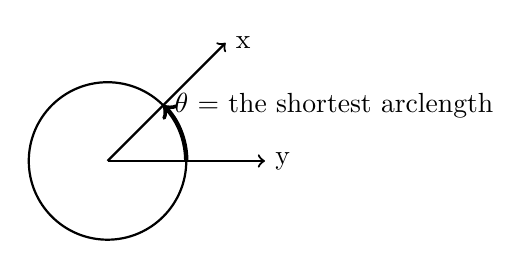
\begin{tikzpicture}
\draw[black, thick](0,0) circle (1);
\draw[black, thick,->] (0,0) -- (2,0) node[anchor=west] {y};
\draw[black, thick,->] (0,0) -- (1.5,1.5) node[anchor=west] {x};
\draw[black, ultra thick, ->] (1,0) arc (0:45:1) node[anchor=west] {$\theta$ = the shortest arclength};
\end{tikzpicture}
}
$cos\theta(\underline{x},y) = \frac{\underline{x}'\underline{y}}{|x||y|} = \frac{\underline{x}'\underline{y}/n}{(|\underline{x}|\sqrt{n})(|\underline{y}|\sqrt{n})}\to \frac{EXY}{\sqrt{EX^2}\sqrt{EY^2}}$\\
\subsubsection{Connection with r}
$\dot{X} = X-EX\quad \dot{Y} = Y-EY$\\
\begin{align*}
	r = \frac{\sum_{i=1}^n(x_i-\bar{x})(y_i-\bar{y})}{\sqrt{\sum(x_i-\bar{x})^2}\sqrt{\sum(y_i-\bar{y})^2}} \stackrel{conv}{\rightarrow}\frac{E\dot{X}\dot{Y}}{\sqrt{E\dot{X}^2}\sqrt{E\dot{Y}^2}} = \frac{E(X-EX)(Y-EY)}{||X-EX||\ ||Y-EY||} = cos \measuredangle(\dot{X}, \dot{Y})
\end{align*}
\begin{definition}
	$cos\angle(x,y)\stackrel{defn}{=}\frac{EXY}{||X||\ ||Y||}\stackrel{LLN}{=}\frac{\underline{x}'\underline{y}}{|x||y|} = cos\measuredangle(x,y)$
\end{definition}
\begin{definition}
	$\rho(x,y) = cos\measuredangle(\dot{X}, \dot{Y}) = \frac{E(X-EX)(Y-EY)}{\sqrt{varX}\sqrt{varY}} = \frac{cov(x,y)}{\sigma(x)\sigma(y)},\quad \sigma(x) = \sqrt{varX} = ||\dot{x}|| = ||X-EX||$
\end{definition}
\subsection{Expected Value}
\begin{ppst}
	EX is the closest constant to X: $||X-EX|| = inf_{t\in \mathbb{R}}||x-t||$
\end{ppst}
\begin{proof}
	hint: f(t) = $\sqrt{E(x-t)^2},\quad g(t) = E(X-t)^2$, try to minimize g(t)
\end{proof}
\subsubsection{properties of $E(\dot{X})$}
\begin{itemize}
	\item $\dot{(X+Y)} =\dot{X}+\dot{Y} =X-EX+Y-EY\\X+Y-E(X+Y) = X+Y-EX-EY$
	\item $(c\dot{X}) = cX-EcX = c(X-EX) = c\dot{X}$
	\item $E\dot{X} = 0$
\end{itemize}
\subsubsection{Expected value for arbitrary finite discrete distribution(Lebesgue-stieltjes)}
$X\sim 
\begin{pmatrix}
	a_1, \cdots, a_n\\
	p_1, \cdots, p_n
\end{pmatrix}\\ \iff x = \sum_{j=1}^N a_jI_{\{a_j\}}(x) \implies EX = \sum_{j=1}^N a_jEI_{\{a_j\}}(x) = \sum_{j=1}^N a_jP(X=a_j) = \sum_{j=1}^Na_jp_j$\\
\\
consider any $\mathbb{R}$-value $x\geq 0$ and let
\begin{align*}
	0\leq x_n &= \sum_{j=1}^n\frac{j-1}{\sqrt{n}}I_{(\frac{j-1}{\sqrt{n}},\frac{j}{\sqrt{n}}]}(x)\leq x\\
	0\leq x-x_n &=\sum_{j=1}^n(x-\frac{j-1}{\sqrt{n}})I_{(\frac{j-1}{\sqrt{n}},\frac{j}{\sqrt{n}}]}(x)+xI_{(\sqrt{n},\infty)}(x)\\
	&\leq \sum_{j=1}^n\frac{1}{\sqrt{n}}I_{(\frac{j-1}{\sqrt{n}},\frac{j}{\sqrt{n}}]}(x)+xI_{(\sqrt{n},\infty)}(x)\\
	&= \frac{1}{\sqrt{n}}I_{(0,\sqrt{n}]}(x)+xI_{(\sqrt{n},\infty)}(x)\\
	&\leq \frac{1}{\sqrt{n}}+xI_{(\sqrt{n},\infty)}(x)\to 0 \text{ as } n\to \infty
\end{align*}
and so we find $x_n\to x $ as $n \to \infty$\\
But now let $h:[0,\infty)\stackrel{cont}{[0,\infty}$(i.e continuous map to real number of non- negative) and we automatically have $h(x_n)\to h(x) \implies Eh(x_n) \to Eh(x)$\\
i.e 
\begin{align*}
	Eh(x_n) &= lim_{n\to \infty}h(\frac{j-1}{\sqrt{n}})p(\frac{j-1}{\sqrt{n}}<x<\frac{j}{\sqrt{n}})\\
	&=lim_{n\to \infty}h(\frac{j-1}{\sqrt{n}})[F(\frac{j}{\sqrt{n}})-F(\frac{j-1}{\sqrt{n}})]\\
	&\stackrel{name}{=}\int_0^\infty h(x)dF(x)\\
	x\geq 0 &\implies xI_{(\sqrt{n},\infty)}(x) = x[\sum_{j=1}^nI_{(\frac{j-1}{\sqrt{n}},\frac{j}{\sqrt{n}}]}(x)+xI_{(\sqrt{n},\infty)}(x)]\\
	&=\sum_{j=1}^nxI_{(\frac{j-1}{\sqrt{n}},\frac{j}{\sqrt{n}}]}(x)+xI_{(\sqrt{n},\infty)}(x)
\end{align*}

\subsection{Covariance}
\subsubsection{Basic Calculation}
\begin{itemize}
	\item $cov(x,y)\stackrel{defn}{=} E\dot{x}\dot{Y} = E(X-EX)(Y-EY)$
	\item $cov(x,x) = EX^2 = E(X-EX)^2 = var(X)$
	\item $cov(X+Y,Z) = cov(X,Z)+cov(Y,Z)$
	\item $cov(cX,Z) = c\ cov(X,Z)$
\end{itemize}
\subsubsection{Three Properties: Bi-linear,Symmetric, non-negative}
\begin{itemize}
	\item bi-linear: $cov(\sum_1^m a_ix_i, \sum_1^n b_jy_j) = \sum_i^m\sum_j^n a_ib_jcov(x_i, y_i)$
	\item symmetrci: $cov(x,y) = cov(y,x)$
	\item non-negative definition: $cov(x,x) = var(x) \geq 0 $ w.eq(with equality) $\iff X\stackrel{defn}{=}EX$
\end{itemize}
\subsection{Markov Inequality and Chebychev Inequality}
\begin{ppst}
	given $Z\geq 0,t\geq 0$, any $g:[0,\infty) \to [0,\infty)$ with $g \uparrow \implies P(Z\geq t)\leq \frac{Eg(Z)}{g(t)} \forall g$ that satisfies all above hypothesis
\end{ppst}
\begin{proof}
	$g(Z)\geq g(t)I(Z\geq t) \implies Eg(Z)\geq EI(Z\geq t) = g(t)P(Z\geq t)$
\end{proof}
\begin{crlr}
	$P(|X-EX|\geq k)\leq \frac{E(X-EX)^2}{k^2}$ i.e $P(|X-EX|\geq k\sigma) \leq \frac{1}{k^2}$
\end{crlr}
application: $varX=0 \iff x \stackrel{wp}{=} EX$
\begin{proof}
	$\\(\implies) \\varX = 0 \implies P(|X-EX|\geq \frac{1}{n})\leq n^2 \times 0=0\\$
	i.e $P(|X-EX|\geq \frac{1}{n})=0 \quad \forall n\\
	P(|X-EX|< \frac{1}{n}) = 1 \quad \forall n\\
	A_n = (|X-EX| < \frac{1}{n})\downarrow$ as $n\to \infty\\
	A = (|X-EX| = 0)\implies P(A_n)\to P(A)$, so $P(A) = 1\\
	P(|X-EX| = 0)=1\\
	|x| = 0 \iff x=0\\$
	equivalently $P(X=EX) = 1$ and so we write $X \stackrel{wp1}{=}EX$ which is merely a symbol for the above.\\
	$(\impliedby)\\P(X=EX) = 1 = P(|X-EX|^2=0)$ so let any $y=(X-EX)^2 = P(y=0)=1$\\
	we find $varX = Ey = 0 \times 1=0$
\end{proof}
\subsection{Conditional Expectation Probability}
Define:
\begin{itemize}
	\item $E(x|w)\stackrel{defn}{=} o.p(X|L_2(w))$ with o.p refers to orthogonal projection and x is R-valued
	\item $L_2(w) = \{g(w)|g: \mathcal{W}\to\mathbb{R}, Eg(w)^2<w\}$
	\item $\mathcal{W} = $ sample space of W
	\item $\mathcal{R}:$ all R-valued random variable
	\item $L_2: $ all R-valued random variable x s.t $Ex^2 < \infty$(Counter Example: take $Z \sim N(0,1), and let x = \frac{1}{z}, x^2 = \frac{1}{z^2}$)
\end{itemize}
Now note $\mathcal{R}$ itself is a vector space. \\
\textbf{Example:} find $cov(\sum_{i=1}^ma_ix_i, \sum_{j=1}^nb_jy_j) = \sum_{i=1}^m\sum_{j=1}^na_ib_j cov(x_i,y_i),$ given $x,y\in L_2$ i.e $Ex^2<\infty, Ey^2<\infty \implies E|XY| <\infty$
\begin{proof}
	$|XY|<\frac{X^2+Y^2}{2}$
\end{proof}
so $EXY\in \mathbb{R}$
\begin{crlr}
	$X,Y\in L_2 \implies X+Y \in L_2$
\end{crlr}
i.e $L_2$ is a sub-vector space
\begin{proof}
	$(X+Y)^2 = X^2+2XY+Y^2\leq X^2+2|XY|+Y^2$ 
\end{proof}
{
\center
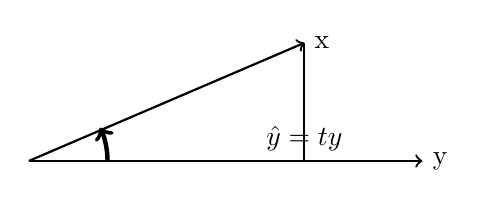
\begin{tikzpicture}
\draw[black, thick,->] (0,0) -- (5,0) node[anchor=west] {y};
\draw[black, thick,->] (0,0) -- (3.5,1.5) node[anchor=west] {x};
\draw[black, thick] (3.5,1.5) -- (3.5,0) node[anchor=south] {$\hat{y} = ty$};
\draw[black, ultra thick, ->] (1,0) arc (0:25:1) ;
\end{tikzpicture}
}
\begin{definition}
	o.p $x|y = \hat{y}$
\end{definition}
This satisfices two properties:
\begin{itemize}
	\item $\hat{y} = ty$ for some $t \in \mathbb{R}$
	\item $x-\hat{y} \bot y \implies E((x-\hat{y})y)=0 \iff E(x-ty)y=0 \iff t = \frac{EXY}{EY^2}$
\end{itemize}
\section{Probability Mass Function(PMF)}
\begin{align*}
	F(x)&=P(X\leq x) = P(X\in(\infty,x)) = P_x(-\infty,x]\\
	F(x+n^{-1}) &= P_x(-\infty,x+n^{-1}] \to F(x)= P_x(-\infty,x]
\end{align*}
we say that any distribution function is not continuous at any point x
\begin{definition}
	$F(x+)=lim_{n\to \infty}F(x+\frac{1}{n}) = F(x)$
\end{definition}
\begin{definition}
	$F(x-) = lim_{x\to \infty}F(x-\frac{1}{n}) = P(X<x)$
\end{definition}
\begin{definition}
	the probability math function of X is $p:\mathbb{R}\to [0,1]$ given by $p(x) = P(X=x)$
\end{definition}
\begin{ppst}
	$p(x) = F(x)-F(x-)$
\end{ppst}
\begin{proof}
	$p(x) = P(X\leq x)-P(X<x) = F(x)-F(x-)$
\end{proof}
\begin{ppst}
	$^{\#}(p>0)\leq ^{\#}N$
\end{ppst}
\begin{proof}
	\begin{align*}
		(p>0) &= \cup_{n=1}^\infty (p>\frac{1}{n})\\
		(p>0) &= p^{-1}(0,\infty) = \{x\in \mathbb{R}|p(x)>0\}
	\end{align*}
	but $\#(p>\frac{1}{n})<n$ because o.w $\exists a_1,\cdots, a_n \in (p>\frac{1}{n})$, so if we let $A = \{a_1,\cdots, a_n\}\implies$ then we find $P(x\in A) = \sum_{i=1}^nP(x=a_i) = \sum_{i=1}^np(a_i)>\frac{n}{n}=1$ 
\end{proof}
e.g let $\mathbb{Q} = \{r_n| n\in\mathbb{N}\}$, let $\{p_n| n \in \mathbb{N}\}$ when $p_n>0$ s.t $\sum_{n\in \mathbb{N}}p_n=1$. We simply define $F(x) = \sum_{\{n|r_n\leq x\}}p_n$
\section{Uniform Distribution}
\begin{definition}
	$U \sim Unif(\Omega),  ^{\#}\Omega <^{\#}\mathbb{N} \quad \iff \quad P(U=\omega) = \frac{1}{^{\#}\Omega}\quad \iff \quad P(U\in A) = \frac{^{\#}A}{^{\#}\Omega}$ 
\end{definition}
e.g 
\begin{align*}
	U &\sim unif \ \{1,\cdots, n\} \iff P(U=i)=\frac{1}{n}, i =1, \cdots, n \\ 
	\text{note that: }\quad -U &\sim unif \ \{-n,\cdots, -1\}\\
	n-U &\sim unif\ \{0,1,\cdots, n-1\}\\
	n-U+1 &\sim unif\ \{1,\cdots, n\}\\
	\begin{rcases}
    n+1-U &\stackrel{d}{=} U\\
    n+1-EU &= EU
	\end{rcases}&\implies EU = \frac{n+1}{2}
\end{align*}
\begin{definition}
	$U\sim unif[0,1] \iff P(U\leq u) = u,\forall\  0 \leq u\leq1$
\end{definition}
\subsection{$U \sim unif\  \{1,\cdots, n\}$, $EU^k-E(U-1)^k = n^{k-1}$}
\begin{itemize}
	\item Since $U \stackrel{d}{=} n+1-U\quad  EU=E(n+1-U) = n+1-EU \implies EU = \frac{n+1}{2} = \frac{1+\cdots+n}{n}$
	\item $U \sim unif \{1,\cdots, n\} \quad U-1 \sim unif \{0,\cdots, n\} \implies$U and U-1 has the similar distribution that differ by a shift.
	\item $U^k\sim unif\ \{1^k,2^k,\cdots, n^k\}\quad EU^k=\frac{1+2^k+\cdots+n^k}{n} \implies E(U-1)^k = \frac{0+1+2^k+\cdots+(n-1)^k}{n}$
	\item $EU^k = \frac{1}{k+1}\quad k \in $
\end{itemize}
\subsection{Variance of U and its calculation}
\textbf{Result}: $Var(U) = Var(U-1) = Var(n+1-U)\frac{n^2-1}{12}$\\
\begin{align*}
	&EU^3-E(U-1)^3 =n^2\\
	&\implies EU^3-(EU^3-3EU^2+3EU-1)=n^2\\
	&\implies 3EU^2 = n^2+3EU-1=(n-1)(n+1)+\frac{3(n+1)}{2} = \frac{(n+1)(2n+1)}{2}\\
	&EU^2 = \frac{(n+1)(2n+1)}{6} = \frac{1+2^2+\cdots+n^2}{n}\\
	\text{recall: } &Var(U) = EU^2-(EU)^2 = \frac{(n+1)(2n+1)}{6}- \frac{n+1}{2}\frac{n+1}{2}\\
	&=(\frac{2n+1}{3}-\frac{n+1}{2})\frac{n+1}{2} = \frac{n-1}{6}\frac{n+1}{2} = \frac{n^2-1}{12}\\
	&\implies Var(U) = Var(U-1) = Var(n+1-U)\frac{n^2-1}{12} \text{ Since }(var(aX+b) = a^2varX)
\end{align*}
\subsection{U and nU}
\subsubsection{$U\sim unif[0,1]\iff [nU]\sim unif\{0,\cdots,n-1\}\forall n$}
\begin{proof}
	$\\ (\implies)\\ P([nU]=k) = P(k \leq nU \leq k+1) = \frac{1}{n}$ provided $k=0,1,\cdots, n-1\\$
	$(\impliedby)\\$to show that $P(U\leq u) = u \quad \forall 0\leq u\leq 1$, consider $P(U>r)$ for any $r \in \mathbb{Q}[0,1)\\$ But
	$P(U <r) = P(nU < k) \text{ for } r = k/n, k<n \\= \sum_{i=0}^{n-1}P(nU<k,[nU]=i) = \sum_{i=0}^{n-1}P(0 \leq nU <k, i\leq nU<i+1)$ \\
	i.e $\cap P \text{ on } [0,k]$ which is the accumulation of P(nU) in each partition\\
	$= \sum_{i=0}^{k-1}P(i\leq nU<i+1) = \sum_{i=1}^{k-1}P([nU]=i)\\
	=k \cdot \frac{1}{n} = \frac{k}{n} = r\\ \implies P(U<r) = r \text{ i.e } P(U\leq u)$ any other $0\leq u <1\\$
	Take $r_n \downarrow u$ at $r_n <1 \quad [0,r_n)\downarrow [0,U]\\P(U<r_n)=r_n \to P(U<u)=u$
\end{proof}
\subsubsection{$U_n \to U$}
$U\sim unif[0,1]\iff nU\sim unif\{0,\cdots,n-1\} \forall n\in \mathbb{N} \implies 0 \leq U-\frac{nU}{n}\leq \frac{1}{n}$\\
so $U_n = \frac{[nU]}{n}\to U$
\section{Bernoulli Distribution}
\begin{definition}
	$Z\sim bern(p) \iff Z\sim \begin{pmatrix}
		0 & 1\\
		q&p
	\end{pmatrix}$, $Z^{-1}\sim \begin{pmatrix}
		\infty & 1\\
		q&p
	\end{pmatrix}$
\end{definition}
note: $Z^s = Z, x>0$

\section{Binomial Distribution}
\begin{definition}
	$X\sim bin(n,p), n \in \mathbb{N}, o\leq p\leq 1 \iff x \stackrel{d}{=}z_1+\cdots+z_n, z_i iid, Z\sim bern(p)$
\end{definition}
\subsection{Properties}
\begin{itemize}
	\item $EX = \sum_1^nEZ_i = nEZ = np$
	\item $VarX=var(Z_1,\cdots, Z_n)\stackrel{indep}{=}VarZ_1, \cdots, VarZ_n+ 0 \cdot cov(Z_i,Z_j) \stackrel{ident}{=}nVarZ=npq $
	\item $\sigma(x) = \sqrt{n}\sqrt{pq}$
\end{itemize}
\begin{ppst}
	$X\sim bin(m,p),Y\sim bin(n,p)\text{ (independent) } \implies X+Y \sim bin(n+m, p)$
\end{ppst}
\begin{proof}
	$Z_1, \cdots, Z_{m+n} \ idd,\ Z\sim bern(p) \implies \begin{pmatrix}
		X\\Y
	\end{pmatrix}\stackrel{d}{=}\begin{pmatrix}
		Z_1+\cdots+Z_m\\Z_{m+1}+\cdots+Z_{m+n}
	\end{pmatrix} \implies X+Y \stackrel{d}{=}\sum_1^{m+n}Z_i$ 
\end{proof}
e.g $g(Z_1, \cdots, Z_n) = \sum_{i=1}^n a_iZ_i^i\implies Eg(Z)=(\sum_{i=1}^na_i)p \quad var g(Z) = (\sum a_i^2)pq$
\subsection{Probability mass function}
$ p(k) = P_k = P(X=k) = P(Z_1+\cdots,+Z_n=k)$ but $P(Z=z) = p^{-z}q^{1-z}, z\in \{0,1\}$
\begin{align*}
	\implies P((Z_1,\cdots,Z_n)=(z_1,\cdots,z_n)) &= P(Z_1=z_1,\cdots,Z_n=z_n)\\
	\stackrel{indep}{=}P(Z_1=z_1)\cdots P(Z_n=z_n) &= p^{z_1}q^{1-z_1}\cdots p^{z_n}q^{1-z_n}\\
	=p^{\sum z_i}q^{n-\sum z_i}\\
	\implies P(X=k) = \sum P((Z_1,\cdots,Z_n)&=(z_1,\cdots,z_n))\quad z_1,\cdots z_n\in C_k^n
\end{align*}
where $C_k^n = \{(z_1,\cdots, z_n)|z_i\in \{0,1\},i=1,\cdots,n\  s.t\ \sum_1^n z_i=k \}$\\
thus
\begin{align*}
	P(X=k) &=\sum_{(z_1,\cdots, z_n)\in C_k^n}p^{\sum_1^nZ_i}q^{n-\sum_1^nZ_i}\\
	&= \sum_{(z_1,\cdots, z_n)\in C_k^n} p^k q^{n-k}\\
	&= p^k q^{n-k}\times ^{\#}C_k^n\\
	&= {n \choose k}p^kq^{n-k}
\end{align*}
\subsubsection{$n\choose k$}
${n\choose k} \stackrel{name}{=}^{\#}C_k^n $\\
$\sum_{k=0}^nP(X=k)=1=\sum_{k=0}^n {n\choose k}p^kq^{n-k} =\sum_{k=0}^n {n\choose k}p^k(1-p)^{n-k}$\\
let $p = \frac{t}{1+t}, q=\frac{1}{1+t}$\\
to find $(1+t)^n = \sum_{k=0}^n{n\choose k}t^k$
\begin{align*}
	n(1+t)^{n-1} &= \sum_{k=0}^n	k{n \choose k}t^{k-1}\\
	\stackrel{also}{=}n\sum_{k=0}^{n-1}{n-1\choose k}t^k &=n\sum_{j=1}^n{n-1\choose j-1}t^{j-1}\\
	&= \sum_{j=1}^n n{n-1 \choose j-1} t^{j-1}\\
	&= \sum_{k=1}^n n{n-1\choose k-1} t^{k-1}
\end{align*}
\begin{thrm}
	$\sum_0^na_kz^k = \sum_0^nb_kz^k \quad z_0-\delta <z <z_0+\delta \iff a_k=b_k \forall k = 0,\cdots, n$
\end{thrm}
\begin{align*}
	\implies k{n\choose k} &= n{n-1\choose k-1} = \frac{n^{(k)}}{k!}\\
	{n\choose k} &= \frac{n}{k} {n-1\choose k-1} = \frac{n(n-1)}{k(k-1)} {n-2 \choose k-2}\\
	&= \frac{n(n-1)\cdots(n-(k-1))}{k(k-1)\cdots (k(k-1))}{n-k\choose 0} = \frac{n^{(k)}}{k!} = \frac{n!}{k!(n-k)!}
\end{align*}
\subsubsection{properties of $n^{(k)}$}
\begin{itemize}
	\item $n^{(k)} = n(n-1)\cdots(n-k+1) = \frac{n!}{(n-k)!}$
	\item $n^{(0)} = 1 = n^0 \quad 0!=1$
\end{itemize}
e.g 
\begin{align*}
	P(X=0) &= {n\choose 0}p^0q^n\\
	&=p(Z_1+\cdots+Z_n=0) = P(Z_1=\cdots=Z_n=0)\\
	&\stackrel{ind}{=} \prod _{i=1}^np(Z_i=0)\stackrel{ind}{=}P(Z=0)^n = q^n
\end{align*}
\subsection{Expected Value}	
\begin{ppst}
	$EX^{(k)} = \begin{cases}
		n^{(r)}p^r &r = 0,\cdots, n\\
		0 &r = n+1,n+2
	\end{cases}$
\end{ppst}
\begin{proof}
	$g(x) = X^{(r)} = x(x-1)\cdots(x-r+1)$ polynomial of degree k, where $x\sim bin(n,p)$\\
	\begin{align*}
		P(X=k)&= {n\choose k}p^kq^{n-k}, k =0,1,\cdots, n\\
		EX^{(r)} &= Eg(x) = \sum_{k=0}^ng(k){n\choose k}p^k q^{n-k}\\
		&= \sum_{k=0}^n k^{(r)}{n\choose k}p^k q^{n-k}\\
		&= \sum_{k=r}^n\frac{k(k-1)\cdots(k-(r-1))n^{(k)}}{k!}p^kq^{n-k}\\
		&= \sum_{k=r}^n \frac{n^{(k)}}{(k-r)!}p^kq^{n-k}\\
		&=\sum_{k=r}^n \frac{n^{(r)}(n-r)!p^r}{(k-r)![(n-r)-(k-r)]!}p^{k-r}q^{(n-r)-(k-r)}\\
		&= n^{(r)}p^r\sum_{k=r}^n {n-r \choose k-r} p^{k-r}q^{(n-r)-(k-r)}\\
		1&= \sum_{k=r}^n {n-r \choose k-r} p^{k-r}q^{(n-r)-(k-r)}\\
		\implies EX^{(r)} &= n^{(r)}p^r
	\end{align*}
\end{proof}
\subsection{Variance}
\begin{itemize}
	\item $EZ^2=EZ=p$
	\item $VarZ = EZ^2-E(Z)^2 = p-p^2 = pq$
\end{itemize}

\section{Negative Binomial \& Geometric Distribution}
\subsection{Definition}
Given
\begin{itemize}
	\item $Z\sim bern(p) \equiv \begin{pmatrix}
		0 & 1\\
		q & p
	\end{pmatrix}$
	\item $Z_i, i\in \mathbb{N}\quad IID Z $
	\item $S_n = \sum_{i=1}^nZ_i, n\in\mathbb{N}\quad S_{n+1} = S_n+Z_{n+1}$
\end{itemize}
\begin{definition}
	$x\sim bern(n,p) \iff x\stackrel{d}{=}S_n$
\end{definition}
\begin{definition}
	$T_k\sim negbin(k,p) \iff (T_k = n) = (S_{n-k} = k-1, Z_n=1), n= k, k+1,\cdots$
\end{definition}
Interpretation of $T_k$: number of trials need to see $k^{th}$ success. 
\begin{definition}
	$W\sim geo(p) \iff W\stackrel{d}{=}T_1, k-1\implies geo(p)\equiv negbin(1,p)$
\end{definition}
\textbf{Note:} $P(W=n)= P(T_1=n) = P(S_{n-1}=0,Z_n=1) = P(S_{n-1}=0)P(Z_n=1) = pq^{n-1}, n=1,2,\cdots$
\begin{ppst}
	$T\stackrel{d}{=}T_k, W \stackrel{d}{=}T_1, T\bot W \implies T+W\stackrel{d}{=}T_{k+1}$
\end{ppst}
\begin{proof}
	\begin{align*}
		P(T+W=n)&=\sum_{i=1}^{n-k}P(T=n-i,w-i) \text{ since } n-i\geq k, i\leq n-k\\
		&=\sum_{i=1}^{n-k} P(T=n-i)P(W=i)\\
		&=\sum_{i=1}^{n-k} P(T_k = n-i)P(T_1=i)\\
		&=\sum_{i=1}^{n-k} P(S_{n-i-1} = k-1, Z_{n-i}=1)P(S_{i-1}=0, Z_i=1)\\
		&=\sum_{i=1}^{n-k} P(Z_1+\cdots+Z_{n-i-1} = k-1, Z_{n-i}=1)^*P(Z_{n-i+1} = \cdots  = Z_{n-1}=0, Z_n=1)\\
		&=\sum_{i=1}^{n-k}P(Z_1+\cdots+Z_{n-i+1}=k-1, Z_{n-i}=1,Z_{n-i+1} = \cdots = Z_{n-1}=0) P(Z_n=1)
	\end{align*}
	Let $j=n-i, i=n-j, \\ 1\leq i\leq n-k, -(n-k)\leq -i \leq-1\\ k \leq n-i \leq n-1, k\leq j \leq n-1$
	\begin{align*}
		&=\sum_{j=k}^{n-1}P(Z_1+\cdots+Z_{j-1} = k-1, Z_j=1, Z_{j+1}=\cdots=Z_{n-1}=0)P(Z_n=1)\\
		P(Z_1+\cdots+Z_{n-1}=k)
		&={n-1 \choose k}p^kq^{n-1-k}\\
		&=\sum_{j=k}^{n-1}P(Z_1+\cdots+Z_n=k, \text{kth success occurs on jth trail})\\
		&=\sum_{j=k}^{n-1}P(Z_1+\cdots+Z_{n-1}=k, Z_1+\cdots+Z_{j-1}=k-1, Z_j=1)\\		
		&=\sum_{j=k}^{n-1}P(Z_1+\cdots+Z_{j-1}=k-1, Z_j=1, Z_{j+1}+ \cdots +Z_{n-1}=0)\\
		&\implies \sum_{n-1}^{j=k}P(Z_1+\cdots+Z_{j-1} = k-1, Z_j=1, Z_{j+1}=\cdots=Z_{n-1}=0)P(Z_n=1)\\ 
		&=P(Z_1+\cdots+Z_{n-1}=k) P(Z_n=1)\\
		&=P(S_{n-1}=k, Z_n=1) \stackrel{defn}{=}P(T_{k+1}=n)	
	\end{align*}
\end{proof}
Application:
\begin{align*}
	T&\stackrel{d}{=} T, W\stackrel{d}{=}T, T\bot W\\
	&\implies T+W\stackrel{d}{=}T_2\\
	T&\stackrel{d}{=} T, W\stackrel{d}{=}T, V\stackrel{d}{=}T \quad (T,W,V) stat ind.\\
	T+W+V\stackrel{d}{=}(T+W)+V
\end{align*}
Thus we see the obvious
\begin{crlr}
	$W_1, \cdots, W_k \ IID, \ W \sim geo(p)\implies W_1+\cdots+W_k \stackrel {d}{=}T_k$
\end{crlr}
\begin{crlr}
	$T_1\stackrel{d}{=}T_{k1}, T_2\stackrel{d}{=}T_{k2}, T_{k1}\bot T_{k2} \implies T_1+T_2\stackrel{d}{=}T_{k1}+T_{k2}$
\end{crlr}
\subsection{Expected value of $T_k$, $S_n$ and $W$}
\textbf{Remember:} $T_k \sim negbin(k,p) \iff (T_k=n)=(S_{n-1}=k-1,Z_n=1) = (S_{n-1}<k<S_n)$\\
$S_n$ = random number of successes in a fixed number n of trails.\\
$T_k$ = random number of trails for a fixed number of k successes.\\
\textbf{Note:} 
\begin{align*}
	ES_n = np;\quad  p=\frac{ES_n}{n}
\end{align*}
p = average number of success per trail.\\
\begin{align*}
	ET_k = \frac{k}{p}, \quad \frac{1}{p} = \frac{ET_k}{k}
\end{align*}
$\frac{1}{p}$ = average number of trail per success
\begin{align*}
	T_k&\stackrel{d}{=}\sum_1^kW_i,\quad W_i IID,\quad ET_k = kEW\\
	EW &=\sum_{n=1}^\infty np(n) = \sum_{n=1}^\infty npq^{n-1} = p\sum_{n=1}^\infty nq^{n-1}\\
	&= p \frac{d}{dq}(\sum_{n=1}^\infty q^n) = p\frac{d}{dq}(\frac{1}{1-q}) = p\frac{d}{dq}(1-q)^{-1} = p(1-q)^{-2} = \frac{1}{p}
\end{align*}
Now, we see a simple connection between $(S_n, n\in \mathbb{N})$ and $(T_k, k\in \mathbb{N})$\\
\textbf{Note:} For instance, $S_m\bot S_n-S_m \forall m<n$ i.e $(Z_1+\cdots+Z_m) \bot (Z_{m+1}+\cdots+Z_n)$
\begin{ppst}
	$T_n>n \iff X_n<k,\quad k\in \mathbb{N},n\in\mathbb{N}$
\end{ppst}
then $T_k\sim negbin(k,p) \iff X_n \sim bin(n,p)$
\begin{proof}
	($\impliedby$) we suppose $X_n\sim bin(n,p) \forall n$\\
	\begin{align*}
		P(T_k=n)&=P(T_k\leq n)-P(T_k<n)\\
		&=P(T_k\leq n)-P(T_k\leq n-1)\\
		&=P(T_k > n-1)-P(T_k > n)\\
		&=P(X_n-1 < k)-P(X_n < k)\\
		&=P(S_n-1 < k)-P(S_n < k)\\
		&=P[(S_{n-1}<k)(S_n<k)^c]\\
		&=P(S_{n-1}<k\leq S_n)\\
		&=P(S_n<k-1, Z_n=1)
	\end{align*}
	($\implies$)
	\begin{align*}
		P(X_n=k) &= P(X_n\leq k) - P(X_n < k)\\
		&= P(X_n < k+1) - P(X_n< k)\\
		&= P(T_{k+1}>n) - P(T_k>n)\\
		&=P(T_k\leq n)-P(T{k+1}\leq n)\\
		&=P(T_k\leq n-1) - P(T_{k+1}\leq n-1)+P(T_k=n)-P(T_{k+1}=0)\\
		&= P(X_{n-1}=k)+P(T_k=n)-P(T_{k+1}=n)\\
		&\stackrel{induction}{=}P(S_{n-1}=k)+P(T_k=n)-P(T_{k+1}=n)\\
		&\stackrel{defn}{=} P(S_{n-1}=k)+P(S_{n-1}=k-1,Z_n=1)-P(S_{n-1}=k, Z_n=1)\\
		&= P(S_{n-1}=k, Z_n=1)+P(S_{n-1}=k, Z_n=0)+P(S_{n-1}=k-1,Z_n=1)-P(S_{n-1}=k, Z_n=1)\\
		&=P(S_n=k)
	\end{align*}
\end{proof}
Thus, $P(T_n>k) = P(S_n<k) =\sum_{i=0}^{k-1}{n \choose i} p^iq^{n-i}$\\
\textbf{Note}
\begin{align*}
	W &\sim geo(p) \iff W\stackrel{d}{=} T\\
	P(W=n) &= pq^{n-1}\quad n  = 1,2,cdots\\
	EW &=\sum_{n=1}^\infty nP(W=n) = \sum_{n=1}^\infty npq^{n-1}\\
	&=p\frac{d}{dq}(\sum_{n=0}^\infty q^n) = p \frac{d}{dq}(1-q)^{-1} = p(1-q)^{-2} = \frac{1}{p}\\
	EW(W-1)&=EW^2-EW\\
	&=\sum_{n=1}^\infty n(n-1)P(W=n) = pq(\sum_{n=1}^\infty n(n-1)q^{n-2})\\
	&=pq+2(1-q)^{-3} = \frac{2q}{p^2}\\
	\text{Thus, } EW^2 &= \frac{2q}{p^2} +EW = \frac{p+2q}{p^2} = \frac{1-q}{p^2}\\
	\text{Therefore, } Var(W) &= \frac{1-q}{p^2} - \frac{1}{p^2} = \frac{q}{p^2}
\end{align*}

\section{Poisson Distribution}
\begin{align*}
	{n \choose k}p^k(1-p)^{n-k}&=\frac{\frac{n(n-1)\cdots(n-k+1)}{n^k}}{(1-\frac{\lambda}{n})^k}\frac{\lambda^k}{k!}(1-\frac{\lambda}{n})^n\\
	\lambda &=np\\
	p &= \frac{\lambda}{n}\\
	\frac{\frac{n(n-1)\cdots(n-k+1)}{n^k}}{(1-\frac{\lambda}{n})^k}&=\frac{1(1-\frac{1}{n})\cdots(\frac{k-1}{n})}{(1-\frac{\lambda}{n})^k}\to 1 \text{, Since } n\to \infty\\
	(1-\frac{\lambda}{n})^n &= e^{-\lambda}
\end{align*}
Thus we define
\begin{definition}
	$N\sim Poisson(\lambda) \iff P(N=k) = lim_{n\to \infty}P(X_n=k) = \frac{\lambda^k}{k!}e^{-\lambda}$ where $X_n \sim bin(n,\frac{\lambda}{n}), (N_t, t>0)$
\end{definition}

\subsection{$N_t$}
$N_t$ = random number of successes in time $t>0$ and we assume:
\begin{itemize}
	\item $N_t\sim Poisson(EN_t)$
	\item $EN_t$ proportional to t
\end{itemize}
\textbf{Note:}$EN = \sum_{k=0}^\infty kP(N=k) = \sum_{k=1}^\infty (\frac{\lambda^{k-1}}{(k-1)!}e^{-\lambda})\lambda = \lambda$ \\
($N_t, t>0$) is a poisson distribution iff
\begin{itemize}
	\item $N_t \sim Poisson(\lambda_t). t>0$
	\item For any $0<t_n \uparrow\uparrow$ as $n\to \infty$ (strictly increasing), $N_{t_1}, N_{t_2}-N_{t_1}\cdots N_{t_n}-N_{t_{n-1}}\cdots$ are mutually statistical independent. 
\end{itemize}

\subsection{$T_n$}
$T_n(n\in \mathbb{N})$ = random amount of time for n successes
\begin{align*}
	T_n>t \iff N_t<n
\end{align*}
Thus, 
\begin{align*}
	1-F_n(t)&=P(T_n>t) = P(N_t<n)\\
	&=[\sum_{k=0}^{n-1}\frac{(\lambda t)^k}{k!}]e^{-\lambda t}	
\end{align*}
so $f_n(t) = F'_n(t) = \lambda \frac{(\lambda t)^{n-1}}{(n-1)!}e^{-\lambda t}$\\
But let $Z_n = \lambda T_n$, to find the pdf for $Z_n$
\begin{align*}
	g_n(Z) &= f_n(t)|\frac{dt}{dz}| = f_n(Z/\lambda)\frac{1}{\lambda}\\
	&= \frac{Z^{n-1}e^{-Z}}{(n-1)!} = \frac{Z^{n-1}e^{-Z}}{\Gamma(n)}
\end{align*}

\section{Gamma Distribution}
\begin{definition}
	$Z\sim Gamma(p), p>0 \iff \ pdf:\frac{Z^{p-1}e^{-Z}}{\Gamma(p)}\ \text{where } \Gamma(p) = \int_0^\infty Z^{p-1}e^{-Z}dz$
\end{definition}
\subsection{$\Gamma(p)$}
\begin{itemize}
	\item $\Gamma(p+1) = p\Gamma(p)$
	\item $\Gamma(n) = (n-1)!$
	\item $\Gamma(\frac{1}{2}) = \sqrt{\pi}$ 
\end{itemize}
\subsection{Gamma and Normal Distribution}
$Z\sim N(0,1) \iff -Z\stackrel{d}{=}Z, \frac{Z^2}{2}\sim G(\frac{1}{2})$
\begin{proof}
	($\implies$)
	\begin{align*}
		let \ w&=Z^2/2\\
		G(W)&=P(W\leq w) = P(-\sqrt{2w} \leq Z \leq \sqrt{2w})\\
		&=2P(0\leq Z \leq \sqrt{2w})\\
		&=2[P(Z\leq \sqrt{2w})-P(Z\leq 0)]\\
		&=2P(Z\leq \sqrt{2w})-1\\
		G(W)& = 2\Phi(\sqrt{2w})-1\\
		\text{Thus, } g(w) &= G'(W) = 2 \phi \sqrt{2w} \frac{\sqrt{2}}{2}w^{1/2-1}\\
		&=\frac{1}{\sqrt{2\pi}}e^{-w}\sqrt{2}w^{1/2-1}, w>0\\
		&=\frac{1}{\sqrt{\pi}}w^{1/2-1}, w>0
	\end{align*}
\end{proof}
\begin{definition}
	$Z\sim G(p), p>0 \iff g(Z) = \frac{Z^{p-1}e^{-z}}{\Gamma (p)}$
\end{definition}
\subsection{Expected Value and Variance}
\begin{align*}
	EZ^s = \frac{\Gamma(p+s)}{\Gamma(p)}
\end{align*}
$Z\sim N(0,1)$
\begin{itemize}
	\item n is odd $\implies -Z^n = (-Z)^n\stackrel{d}{=}Z^n \implies -EZ^n = EZ^n \implies EZ^n = 0$
	\item n is even $\implies \text{since } Z^2 = 2W, W\sim G(\frac{1}{2}) \implies Z^n = Z^{2k} = 2^kW^k$
	\begin{align*}
		EZ^n &= 2^kEW^k\\
		&=\frac{2^k\Gamma(k+\frac{1}{2})}{\Gamma(\frac{1}{2})}\\
		&=2^k\frac{\frac{2k-1}{2}\Gamma(\frac{2k-1}{2})}{\Gamma(\frac{1}{2})}\\
		&=\text{Product of all the odd numbers below n}
	\end{align*}
	E.g $Z\sim N(0,1), EZ^6 = 15\cdot 13\cdot 11\cdot 9\cdot 7\cdot 5 \cdot 3$ for n=odd
	\item $Var(Z^2) = EZ^4-(EZ^2)^2 = 3-1=2$
\end{itemize}
\begin{ppst}
	$T = Z+W, U = Z/T \text{ then }Z\sim G(p), W\sim G(p),Z\bot W \iff $
	\begin{itemize}
		\item $T\sim G(p+q)$
		\item $f_u(u) = \frac{\Gamma(p+q)}{\Gamma(p)+\Gamma(q)}u^{p-1}(1-u)^{q-1}, 0<u<1$
		\item $T\bot U$
	\end{itemize}
\end{ppst}
\begin{proof}
	\begin{align*}
		g(z,w) &=\frac{Z^{p-1}e^{-Z}W^{q-1}e^{-W}}{\Gamma(p)\Gamma(q)}\\
		h(u,t) &= g(z,w)|\frac{\partial(z,w)}{\partial(u,t)}|_+\\
		|\frac{\partial ut, (1-u)t}{\partial u,t}|_+ &= \begin{bmatrix}
			t &u\\
			-t & 1-u
		\end{bmatrix}_+ = t\\
		h(u,t) &= \frac{\Gamma(p+q)}{\Gamma(p)\Gamma(q)}u^{p-1}(1-u)^{q-1}\frac{t^{p+1-1}e^{-t}}{\Gamma(p+q)}
	\end{align*}
\end{proof}

\section{Beta Distribution}
\begin{definition}
	$U\sim beta(p,q) \iff U = \frac{Z}{Z+W}, Z\sim G(p), W\sim G(P), Z\bot W$
\end{definition}
Notice that with 
\begin{align*}
	T = Z+W &\implies Z^2 = U^2T^2\\
	\text{so, } EZ^2 &= EU^2ET^2, \text{using independent}\\
	\text{so, } EU^2 &= \frac{EZ^2}{ET^2} = \frac{\Gamma(p+2)/\Gamma(p)}{\Gamma(p+q+2)/\Gamma(p+q)}\\
	EU &=\frac{EZ}{ET} = \frac{p}{p+q}\\
	Z&\sim G(p), EZ^s = \Gamma(p+s)/\Gamma(p)\\
	EZ &= p = Var(Z)\\
	EZ^{-1} &= \Gamma(p-1)/\Gamma(p) = \frac{1}{p-1}\\
	E(Z/W)&=E(ZW^{-1}) = EZEW^{-1} = p\frac{1}{q-1} = \frac{p}{q-1} 
\end{align*}

\section{$\chi^2$ Distribution}
$\chi_{(m)}^2 = 2Z, Z\sim G(m/2)$\\
Since $Z_1, \cdots, Z_n$ IID $Z\sim N(0,1)$ and $\frac{Z_1^2}{2},\cdots, \frac{Z_n^2}{2}$ IID $\frac{Z^2}{2}\sim G(\frac{1}{2}) \implies \frac{2\sum Z_i^2}{2} \sim 2G(\frac{n}{2}) = \chi_{(n)}^2$

\section{Additional Definitions}
\begin{definition}
	$Z\sim N(0,1), \phi(Z) = \frac{1}{\sqrt{2\pi}}e^{-Z^2/2}$
\end{definition}
\begin{definition}
	$X\sim N(\mu,\sigma^2) \iff X = \mu+\sigma Z$
\end{definition}
\begin{definition}
	$Z \sim exp(1) \iff f(Z) = e^{-Z}$
\end{definition}
\begin{definition}
	$X \sim exp(\theta) \iff X = \theta Z$
\end{definition}
\begin{definition}
	$Z\sim G(p) \iff f(Z) = \frac{z^{p-1}e^{-Z}}{\Gamma(p)}$ and $X\sim G(p,\theta) \iff X = \theta Z$
\end{definition}
Thus, $EX^s = E(\theta Z)^s = \theta^sEZ^s = \frac{\theta^s \Gamma(p+s)}{\Gamma(p)}$
\end{document}
